\documentclass[showcase, preprintnumbers, amsmath, amssymb, bibnotes, 12pt]{revtex4} 
\usepackage{natbib}
\usepackage{bm} 
\usepackage{textcomp}
\usepackage{wasysym} 
\usepackage{verbatim}
\usepackage{rotating} 
\usepackage{epsfig} 
\usepackage{graphicx}
\usepackage{subfigure}

\begin{document}

\title{Exploring Morphological Parameters in the Fundamental Plane Space of Quiescent Galaxies}
\author{Anthony A. Paredes}
\affiliation{University of California, Berkeley}
%\author{Genevieve Graves}
%\affiliation{University of California, Berkeley}
\date{Spring 2012}

\begin{abstract}
\begin{center}
ABSTRACT
\end{center}
With the use of data from the Sloan Digital Sky Survey, $\sim 14,000$ quiescent galaxies in red shift, $z$, range of $0.025\leq z\leq0.100$ were examined in Fundamental Plane (FP) space. By separating these galaxies into both disc and bulge morphological types though use of an automated classification algorithm, the spectra of galaxies sharing similar FP parameters ($R_e, \sigma$, and  $I_e$) were stacked to optimise the signal to noise ratios in measurements the stellar population parameters of Age, [Fe/H], and [Mg/Fe] for these galaxies. The stars in the central regions of the galaxies of different morphological type sharing similar values of their FP parameters showed no statistically significant differences in their stellar population parameters. This suggests that there is not strong evidence supporting ideas of a passive red disc phase of galaxy evolution, going from being a spiral galaxy in the blue cloud to an elliptical galaxy in the red sequence, since the ages of the stellar populations appear to be similar for both red disc and red bulge morphological types.
\end{abstract}



\maketitle

\section{Introduction}

Galaxies are known to populate a bimodal colour distribution which is separated into the blue cloud and the red sequence. The blue cloud contains galaxies which appear blue in colour and tend to have on going star formation. The red sequence contains the galaxies where star formation has been quenched (Strateva et al. 2001; Baldry et al. 2004; Gomez et al. 2003). Astronomers believe that there is some physical process that quenches star formation in the blue cloud (Faber et al. 2007). %For example, SOANDSO suggest that the quenching process comes from mergers which then form into bulge type, red sequence galaxies. 

In this paper, we compare the stellar population properties between different morphological types. A galaxy's morphology is, in essence, the galaxy's shape. It has been a known phenomenon in galactic astrophysics for decades, dating back to as early as Hubble's tuning fork evolutionary model, that  galaxies have different morphological types. Galaxies which populate the blue cloud are typically Sa, Sb, Sc, and Irr type galaxies while E and S0 galaxies are mostly found to populate the red sequence (Strateva et al. 2001). We will be making comparisons between bulge (E) and disc (S0) type galaxies in the red sequence. Bulge type galaxies are ellipticals which are dominated by a central spherical bulge and whose light profile fit well with a de Vaucouleurs profile. %(REF)
 Disc type morphological galaxies are typically of type S0 and have a light profile well described by a exponential fit.%(REF) 

It is thought that galaxies evolve such that they migrate from the blue cloud to the red sequence (Faber et al. 2007). Since galaxies in the blue cloud tend to be spirals, and galaxies in the red sequence tend to be ellipticals, it is suggested that morphological change, or going from a spiral morphology to an elliptical morphology, goes hand-in-hand with quenching of star formation, or becoming red in colour.

Not all galaxies follow the trend between morphology and colour. For example, astronomers have observed blue elliptical galaxies (Schawinski et al. 2009). Also, S0 galaxies are part of the population that make up the red sequence and have disc type morphology. Since the processes that are responsible for the quenching of star formation are not completely understood, the stellar properties of the blue ellipticals and red disc can give insight to the quenching process. 

Bundy et al. (2010) propose that red disc galaxies are a step in the evolutionary sequence. To test this theory, we will compare the stellar populations of red disc and red, bulge dominated, ellipticals. One specific stellar population property we will measure is the age of the stars in the two galaxy populations. If the red discs have younger stars then the red ellipticals, then we can confirm the proposal of Bundy et al. (2010).

\section{Data}

In order to obtain a sample selection of quiescent galaxies, the Sloan Digital Sky Survey (SDSS, York et al. 2000)
% data release ??????????????????? 
was used. 

With this data selection, only galaxies between a redshift($z$) of $0.025\leq z\leq0.100$ were chosen for a variety of reasons. The low end of $z$ was chosen because we used the spectral feature of 0II emission lines as a way of selecting non-star forming galaxies. The SDSS spectrograph takes measurements down to wavelengths of 3800$\ \text{\AA}$, since OII has emission at 3727~$\ \text{\AA}$, having a low end of $z$ at 0.025 makes sure that we can see the OII feature. The specific value for $z$ on the high end ($0.100$) was chosen so that we had only a small slice of cosmic time and would not have to worry about evolution on cosmological timescales.

Since we only wanted to explore the properties of quiescent galaxies, selections for these types of galaxies had to be made. If a spectrum from SDSS measured an $ 0.8\ \text{\AA} \leq \text{EW}_{\text{H}\alpha} \leq 2.0\ \text{\AA}$ and/or an EW$_{\text{OII}} \leq 2.00\ \text{\AA}$, then the galaxy was kept in the sample. The others were removed.
 %WE MAY HAVE TO GO INTO MORE DETAIL ABOUT THE $EW$ MEASUREMENTS.

Additional cuts were made for purposes of assuring that our data sample was of the highest quality possible. The first cut was to remove any galaxy with a $u$, $g$, $r$, $i$, and/or $z$ absolute magnitude that was not able to be measured by SDSS.
%(DATA TABLE LISTED NaN). 
The other quality cut was to remove any galaxy in the sample whose value for velocity dispersion, $\sigma$, did not fall in the range $70.0\  \text{km/s} \leq \sigma \leq 300.0\  \text{km/s}$. There are two reasons for the cuts on $\sigma$, one reason for the high end and a separate reason for the low end. The reason to only keep galaxies with a value for $\sigma \geq 70.0\ \text{km/s}$ is due to the resolution of the SDSS spectrometer. In ranges of $\sigma \leq$ 70.0 km/s the width of a spectroscopic line is more as a result of the resolution and not intrinsic $\sigma$ of the target galaxy. The purpose of removing galaxies with $\sigma \geq 300.0\ \text{km/s}$ is because it has been shown that typically galaxies will not have values for $\sigma$ in this range. When it is measured, it is usually a result of another factor, e.g., Berandi et al. (2006) claim that it is a result of background galaxies' relative motions.

To be certain that the cuts on the galaxy properties did in fact give us a sample of quiescent galaxies, a colour magnitude diagram was examined. Figure~\ref{fig:color_mag} shows a plot of the colour magnitude diagram. The red data points represent the galaxies kept in our sample while the contour lines represent the density of all galaxies from the specified SDSS release in the $z$ range $0.025\leq z\leq0.100$. As one can see, the galaxies kept in the sample for analysis resides in the red sequence, while the galaxies in the blue cloud have been removed. 


\begin{figure}
\begin{center}
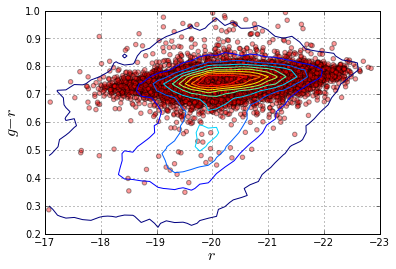
\includegraphics[scale=0.73]{color_mag.png}
\end{center}
\caption{A colour magnitude diagram for the galaxies in $z$ range $0.025\leq z\leq0.100$. The red points represent galaxies kept in our sample while the contour lines represent the density of points where all of galaxies' data points would have been found. As one can see, some galaxies from the blue cloud have made it into our data sample. By analyzing thumbnail photographs from the SDSS imaging tool, we noticed that the galaxies appear blue in colour, but the central bulge region of these galaxies is red in colour. This means that keeping these $\sim50$ galaxies in our sample is acceptable since we only looked at the properties of the stars in the central bulge regions of different morphological types.
% Few galaxies that were not chosen are apparently part of the red sequence; this is because galaxies were chosen to not have \emph{emission} lines, which means that LINERS which are typically red in color NEED REFERENCE, were removed from the sample. 
\label{fig:color_mag}} 
\end{figure}


% Of course one may see that there are some galaxies in the red sequence that have been removed. This is because we chose galaxies based on emission. These red galaxies with emission could be LINERS, which would pollute our sample. 

% Not being measured by SDSS gave value of NaN for magnitudes
\subsection{Morphological Data}

One property that we looked at in our galaxy sample was each galaxy's morphology. In order to do this properly we had to have data about the galaxy's physical appearance.

The light concentration ($C$) of the galaxy is a bit of data that we used. The concentration is a measurement defined by the ratio of the radius in which 90\% of the light of the galaxy is contained ($R90$) to the radius in which 50\% of the light is contained ($R50$). In mathematical terms, $C=R90/R50$.

The ratio of the semi-minor axis to the semi-major axis, $b/a$, was also used for morphological purposes. %HOW ARE THESE MEASURED?

\subsubsection{GIM2D}

There are two parameters used, defined by Simard et al. (2002), known as the bulge light fraction ($B/T$) and the smoothness parameter ($s2$). To measure $B/T$ is to fit the light profile of a galaxy as (disc) exponential profile and a (bulge) de Vaucouleurs profile. Then $B/T$ is calculated by taking the flux of the bulge component of a galaxy to the flux of the sum of the bulge and disc components. 

To measure $s2$, one needs to use a residual image. A residual is defined by a galaxy image minus a smooth model fit. $s2$ is then defined as the sum of two residuals called the total residual ($R_T$) and the asymmetric residual ($R_A$). These are defined in Simarad et al. (2002) as

\begin{equation}
R_T = \frac{\Sigma (1/2)|R_{ij} + R_{ij}^{180}|}{\Sigma I_{ij}} - \frac{\Sigma (1/2)|B_{ij} + B_{ij}^{180}|}{\Sigma I_{ij}}
\label{eq:total_residual}
\end{equation}

\noindent and

\begin{equation}
R_A = \frac{\Sigma (1/2)|R_{ij} - R_{ij}^{180}|}{\Sigma I_{ij}} - \frac{\Sigma (1/2)|B_{ij} - B_{ij}^{180}|}{\Sigma I_{ij}},
\label{eq:asymmetric_residual}
\end{equation}

\noindent where $R_{ij}$ is the pixel value of an object pixel in the residual image, $I_{ij}$ is the pixel value in the full image, $B_{ij}$ is the value of a random background pixel of the full image, and $R_{ij}^{180}$ and $B_{ij}^{180}$ are corresponding galaxy and background pixel values in the residual image after a 180 degree rotation about the galaxy's centre.

\section{Morphological Classification}

To separate the quiescent galaxy sample into different morphological types, we separated the galaxies into three types of morphologies: disc, bulge, and intermediate. The parameters used to do this were the GIM2D parameters, $B/T$ and $s2$, the Concentration, and $b/a$.

In order for a galaxy to be considered a bulge type galaxy, it had to meet the following criteria:

\begin{enumerate}
\item $B/T > 0.5$
\item $s2 \leq 0.08$
\item $b/a > 0.65$
\item $C > 2.9$.
\end{enumerate}

For a galaxy to be considered a disc type galaxy, it is a bit more complicated. If it did not meet the $B/T$ criteria of a bulge type, it is classified as a disc. If it did meet the $B/T$ criteria of a bugle type, but not the $s2$ criteria, it was also classified as a disc. If the galaxy met the bulge type classification criteria for $B/T$ and $s2$, but had a measurement of $b/a \leq 0.45$, the galaxy was classified as a disc morphological type.

All other galaxies were classified as intermediate morphological types.

The way the galaxies were separated is discussed in detail in Cheng et al. (2011). More specifically, Figure 10 of Cheng et al. (2011) is an excellent graphical representation of the decision tree described above.

Sample images for bulge type and disc type galaxies can be found in Figures~\ref{fig:disk}~and~\ref{fig:bulge}, respectively. In this random selection of galaxies, it is apparent that the classification tree has worked. The images in Figure~\ref{fig:disk} show galaxies that have disc components, while the images in Figure~\ref{fig:bulge} show bulge dominated galaxies. One may also notice, that, although the galaxies in Figure~\ref{fig:disk} are disc morphological types, they do contain a large central bulge. Furthermore, Figures \ref{fig:disk} and \ref{fig:bulge} emphasize that the galaxy sample used in the analysis of this paper are red in colour, again confirming that these are galaxies that have quenched stellar formation processes.

\begin{figure}
\begin{center}
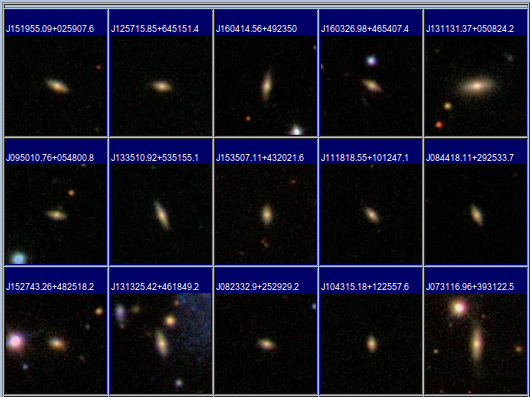
\includegraphics[scale=0.73]{disk.png}
\end{center}
\caption{A few example images of quiescent galaxies that were classified as having disc type morphologies. It is noted only that these do appear to have bulges in their centres and contain disc components.  They also appear red in colour, reinforcing our confidence that the galaxies in our sample are quiescent. \label{fig:disk}} 
\end{figure}


\begin{figure}
\begin{center}
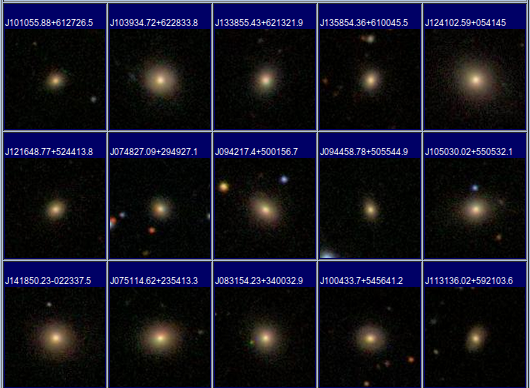
\includegraphics[scale=0.73]{bulge.png}
\end{center}
\caption{Example images of quiescent galaxies that were classified as having bulge type morphologies. As one can see, there is no disc component to any of these galaxies; they are completely bulge dominated. Furthermore, we reinforce that our data sample only contains galaxies whose central region are non star forming due to the fact that the images of these galaxies appear red in colour. \label{fig:bulge}} 
\end{figure}


\section{The Fundamental Plane}

In order to explore the how stellar population parameters varied between morphological types, it was important to explore the difference between them while other parameters were still kept the same. In order to insure this, fundamental plane (FP) space was used. %The FP is traditionally a way of measuring distances. It is a relation between the effective radius, $R_e$, which is the radius of a galaxy in which 50\% of the light is enclosed, the effective surface brightness, $I_e$, the luminosity per unit are within $R_e$, and the velocity dispersion $\sigma$.

Early-type, or quiescent galaxies are known to populate a three-dimensional (3D) parameter space known as the Fundamental Plane (FP; Djorgovski \& Davis 1987). The FP is comprised of a galaxy's central velocity dispersion ($\sigma$), the effective radius ($R_e$), defined to be the radius where half of the galaxy's light is enclosed, and the effective surface brightness ($I_e$), the luminosity per unit area of the galaxy enclosed by $R_e$. If a mass to light ratio ($M/L$) were to be assumed to be of unity, a relation of $R_e \propto \sigma^2I_e^{-1}$ can be derived from the virial theorem. In actuality, the FP has been shown to be $R_e \propto \sigma^{1.24}I_e^{-0.82}\ $(J\o rgensen et al. 1996). There have been multiple explanations for the tilt, e.g., Graves \& Faber (2010) show that the $M/L$ can vary amongst galaxies. 

Exploring the galaxy stellar populations in FP space is a good choice to make. In Graves et al. (2010), the trends of age and metallicity across the FP were analyzed for red sequence galaxies. In a way, this paper is an extension of that work, now adding a 5$^{\text{th}}$ dimension to analyze. That is, we are adding a dimension of morphological type on top of the existing four: $R_e$, $I_e$, $\sigma$, and a stellar population property.

Another reason why choosing FP space is a good idea is that in our analysis, we wanted to make sure we were determining how stellar population properties compared between the different morphological types. Since we already know that the properties vary as a whole across the FP (Graves et al. 2010), it will be important to know how the different morphological types within the same section of the FP vary among stellar population parameters. 

For our chosen set of quiescent galaxies, the FP relation is given by 

\begin{equation}
I_e \propto \sigma^{1.24} {R_e}^{-1.99}. 
\label{eq:FP_prop}
\end{equation}

\noindent The mathematical method used to fit the function to the plane was the method known as least square fitting. The least square fitting was performed on a linear function of the parameters in logarithmic space to be $\log I_e = -1.19 \log R_e + 1.24 \log \sigma + 0.18$. This gives rise to the proportionality given by equation~\ref{eq:FP_prop}. See Figure~\ref{fig:FP_morph} to view a plot of the FP, and in the figure, note that the different morphological types are represented by different colours. Red points are bulges; green points are intermediates; blue points are discs. As one can see, the three different morphological types populate the same parts of the FP, with the disc having the most overall spread.

\begin{figure}
\begin{center}
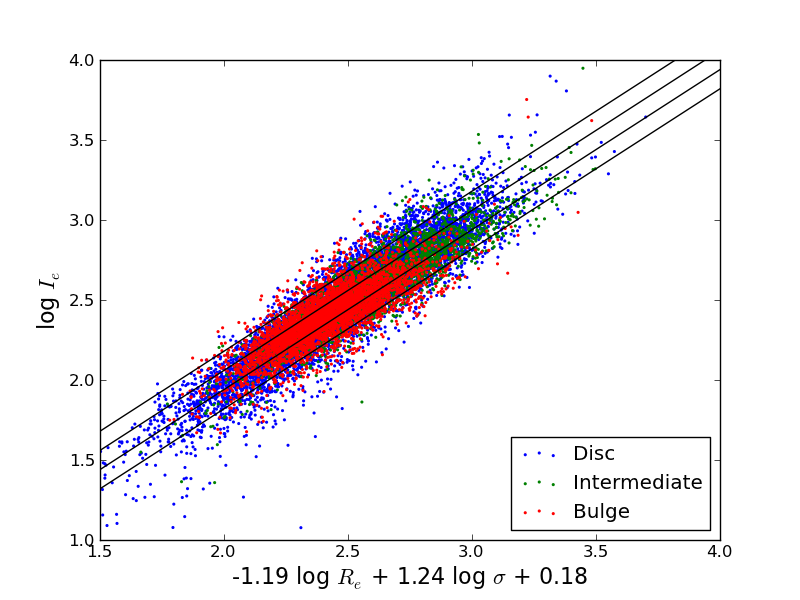
\includegraphics[scale=0.73]{FP_morph.png}
\end{center}
\caption{The FP as seen edge on. Through least square fitting, the FP is given by $\log{I_e}=-1.19\log{R_e}+1.24\log{\sigma}+0.18$. The diagonal lines are a way to represent how the different slices in $\Delta\log{I_e}$ are separated. The three regimes of $\Delta\log{I_e}$ are defined by $-0.18\le\Delta\log{I_e}\le-0.06$ being low-SB, $-0.06<\Delta\log{I_e}<0.06$ being the midplane, $0.06\le\Delta\log{I_e}\le0.18$ being high-SB. Blue, green, and red points represent disc, intermediate and bulge type galaxies respectively. \label{fig:FP_morph}}
\end{figure}

To further dissect the FP, we then split it into three different slices of $\Delta\log{I_e}$ where low-SB(Surface Brightness), mid-SB, and high-SB are where $-0.12\leq\Delta\log{I_e}\leq-0.06$, $-0.06\leq\Delta\log{I_e}\leq~0.06$, and $0.06\leq\Delta\log{I_e}\leq0.12$ respectively. The parameter $\Delta\log{I_e}$ is a measurement of how different the measured value of the surface brightness of a galaxy varies with respect to the expected value that would be calculated using the fundamental plane formula. The black lines in Figure~\ref{fig:FP_morph} represent different sections of $\Delta~\log~I_e$; we will use these different sections later to aid us with the dissection of the FP. A further dissection of the FP is shown in Figure~\ref{fig:FP_split_morph}. This figure is very telling of how the different morphologies populate the FP. With the same colour assignment as Figure~\ref{fig:FP_morph}, the top row are the disc type galaxies represented with blue points, the middle row contains the intermediate galaxies represented by green points, and the bottom row contains the bulge type galaxies represented by red points. Each column represents a different portion of surface brightness with the rightmost being low-SB, the middle row being mid-SB and the leftmost as high-SB. Each of the nine panels is a scatter plot of $\log{\sigma}$ on the horizontal axis and $\log{R_e}$ on the vertical axis. 

\begin{figure}
\begin{center}
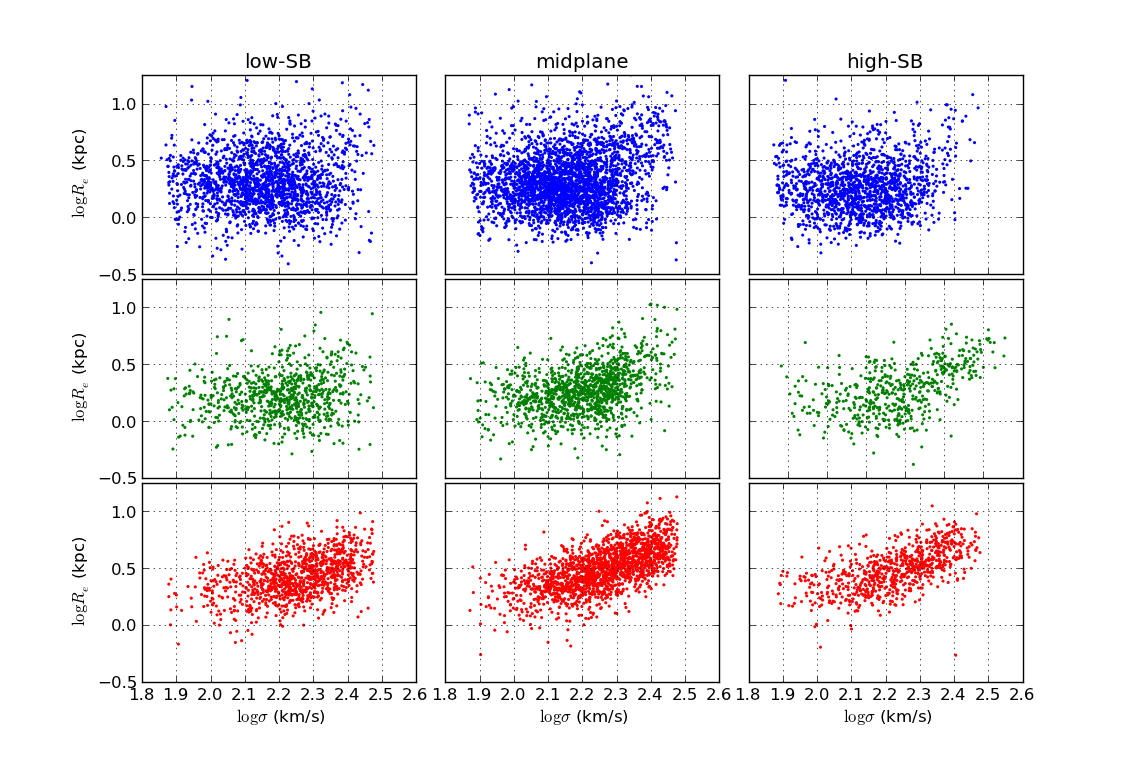
\includegraphics[scale=0.63]{FP_split_morph.png}
\end{center}
\caption{The FP split into the three regimes of surface brightness as defined by the diagonal lines in Figure~\ref{fig:FP_morph}. The red points represent the bulge morphology type galaxies, green represents the intermediates, and blue represents the disc type morphological galaxies. The leftmost column represents the low-SB galaxies, the middle column contains the mid-SB galaxies and the high-SB galaxies are in the rightmost column. In each of the 9 panels, the vertical axis is $\log{R_e}$ and the horizontal axis is $\log{\sigma}$.  \label{fig:FP_split_morph}} 
\end{figure}

Since it can be shown through the virial theorem that the dynamical mass ($M_{dyn}$) varies with the FP parameters as $M_{dyn}~\propto~\sigma^2~R_e$, more massive galaxies will populate the upper-right corner of each of the nine panels of Figure~\ref{fig:FP_split_morph}. This means the bulge types show to dominate the population in the high $M_{dyn}$ portion of the FP while the disc type galaxies tend to show a higher population density in the low $M_{dyn}$ portion. Furthermore, this plot goes on to show how the classification decision tree of how to classify morphological types is a good way of classification, since the intermediate type galaxies populate a section of the FP that would have a $M_{dyn}$ in between the dynamical masses of disc and bulge morphological types. 


\section{Results}


For each of the stellar population parameters, the value that we analyzed is the difference of the parameter for the disc type galaxies that lie in a specific part of the FP to that of the bulge type in the exact same part of the FP. To do this, the FP was split into 192 pieces: three slices of surface brightness, 8 even slices of $\log{\sigma}$, and 8 even slices of $\log{R_e}$. Since not every section contained enough galaxies of a certain type of morphology to carry out the stacked-spectral analysis, not every portion of the FP was able to be examined.

To measure the different stellar population parameters, the spectra in each bin of the FP was stacked in order to have an optimal signal to noise (S/N) ratio. Using the package \emph{EZ\_Ages}\footnote{astro.berkeley.edu/\texttt{\~}graves/ez\_ages.html} the age, [Fe/H], and [Mg/Fe] stellar parameters were measured. See Graves \& Schiavon (2008) for the methods described in doing this.

\subsection{Age}

By using the H$\beta$ spectral line, the age of the galaxies was measured for the galaxies in each of the FP sections described above. A colour representation of the values measured is shown in Figure~\ref{fig:age_maps}. 


\begin{figure}
\begin{center}
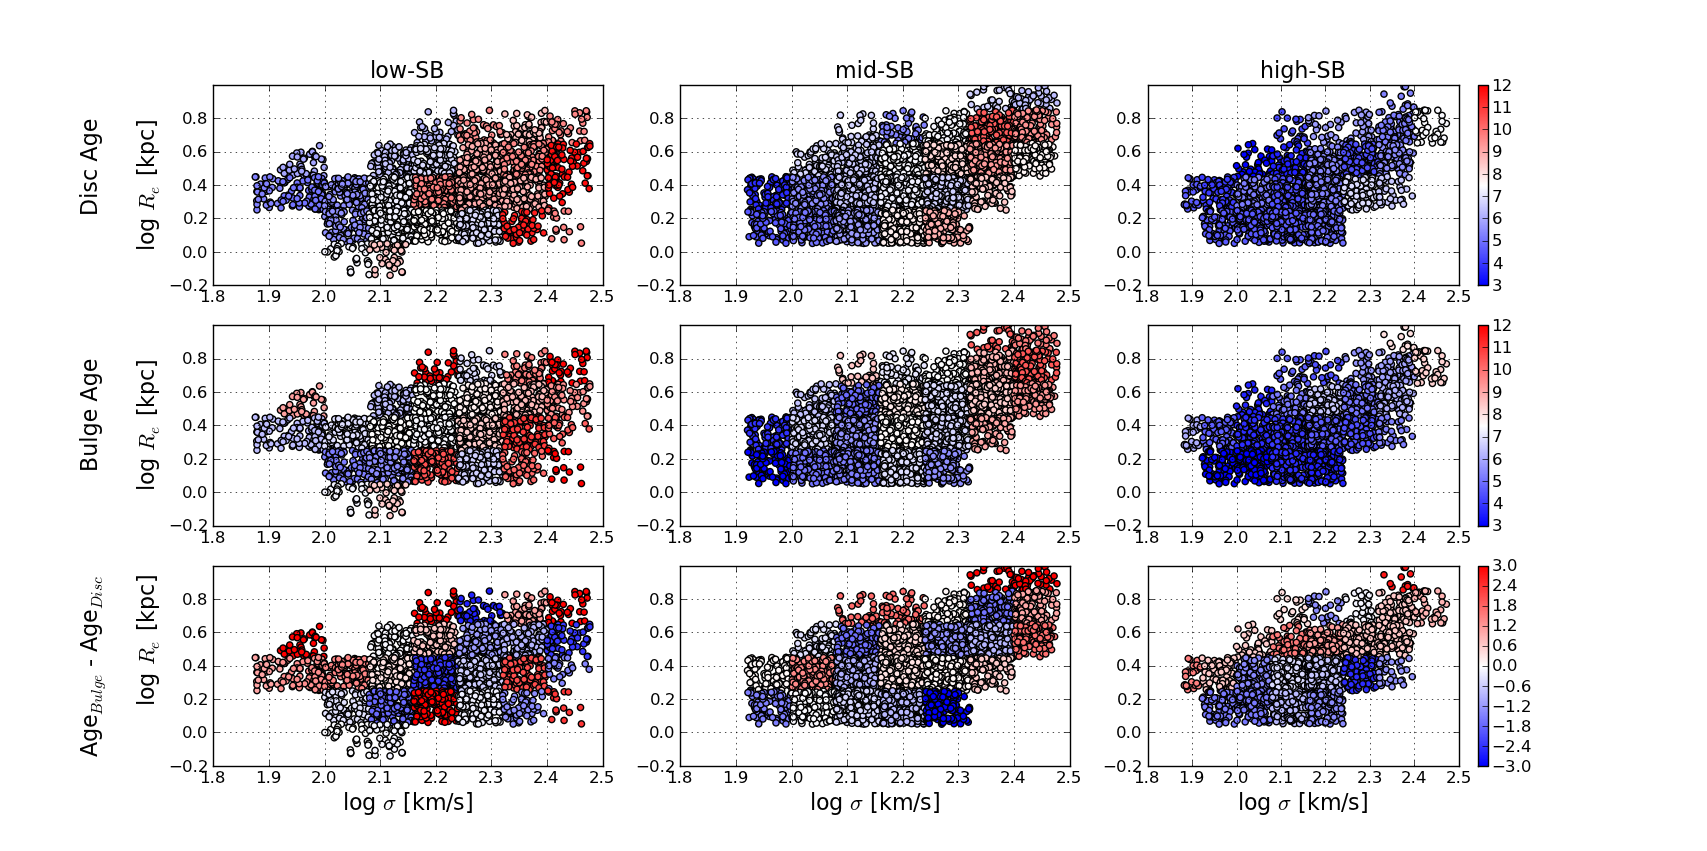
\includegraphics[scale=0.43]{Age_map_9panel.png}
\end{center}
\caption{This figure shows the measurements for the ages of the galaxies in each section of FP space. The ages of theses galaxies were measured using the H$\beta$ spectral line. Columns 1, 2, and 3 represent the low-, mid-, and high-surface brightness sections of the FP respectively. The bluer a data point, the younger it is, while red represents older galaxies. The first and second rows represent the disc and bulge morphological type galaxies respectively. The trends explored in Graves' thesis papers are still present, with brighter galaxies being younger, and galaxies with larger dynamical masses, i.e., larger values of $R_e$ and $\sigma$ are typically older. When examining the difference in the measured ages between the disc and bulge morphological type galaxies (row 3), one can see that there is zero difference between the two, on average, while keeping all other FP parameters the same. \label{fig:age_maps}}
\end{figure}

For both disc and bulge morphological type galaxies, it can be seen that the expected trends are still present, with the brighter galaxies being typically younger and the more massive galaxies having older ages. But when comparing the disc to the bulge morphological types from the same part of the FP, we see that the ages are the same for the stellar populations at the center of these galaxies. When creating a distribution of the difference in age between disc and bulge types where each sample is from each section of the FP described above, the mean value is $0.162\pm0.024$ Gyr with a standard deviation of 1.655 Gyr. A histogram of this distribution can be seen in the first panel of Figure~\ref{fig:Delta_hist}.

\subsection{[Fe/H]}

%SHOULD I GO INTO WHAT [Fe/H] TELLS US ABOUT THE GALAXY'S STARS HERE.  

The iron abundances, [Fe/H], of the galaxies in our sample was also measured. It shows in Figure~\ref{fig:FeH_maps} that the trends already known to exist are present. That is, [Fe/H] does not depend on $R_e$, and that it increases with $I_e$ and $\sigma$. What is interesting is shown quantitatively by means of a histogram in the second panel of Figure~\ref{fig:Delta_hist}. What this is showing is that the difference in [Fe/H] between disc and bulge morphological types, where the FP parameters are the same, are not statistically significant. The distribution samples represent the different sections of the FP. It has a mean value of $0.050\pm0.001$ with a standard deviation of 0.099. Therefore, it can be stated that in the central parts of quiescent galaxies, the iron abundances do not have any correlation to the morphological type.  

\begin{figure}
\begin{center}
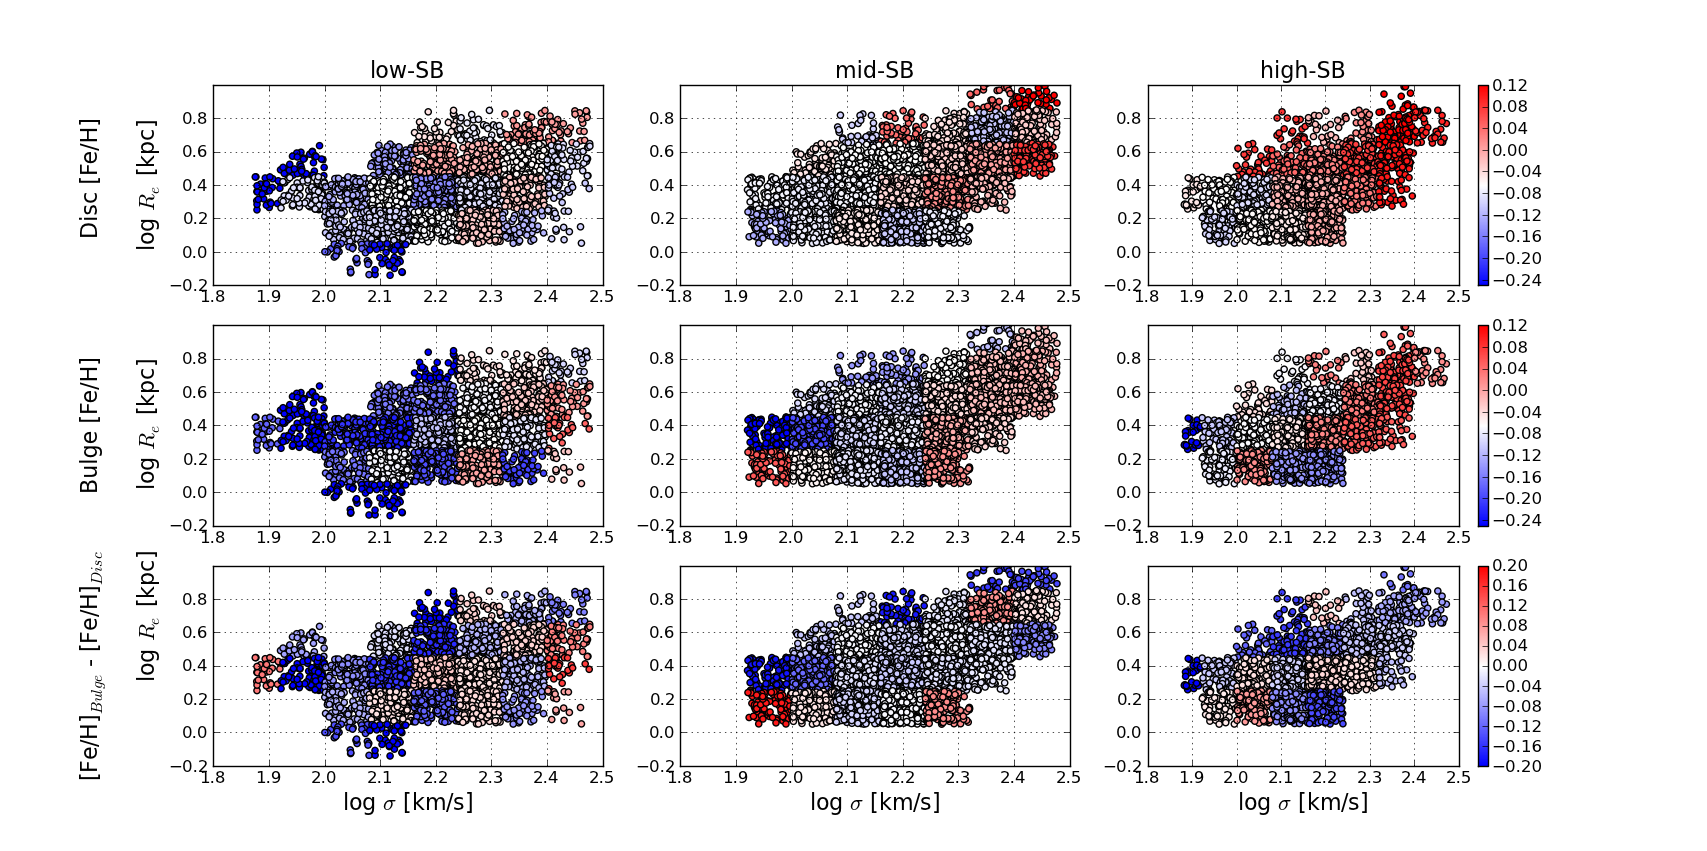
\includegraphics[scale=0.43]{FeH_map_9panel.png}
\end{center}
\caption{The [Fe/H] metallicities of the galaxies are explored in the above figure. Columns 1, 2, and 3 represent the low-, mid-, and high-surface brightness section of the FP, respectively. The redder a point is, the more iron rich the galaxies in that part of the FP are. It shows that galaxies with a larger $I_e$ tend to be more iron rich, and galaxies with large values for $\sigma$  tend to contain more iron as well. Furthermore, iron abundances do not show any relationship with $R_e$, being nearly constant for all $R_e$ with fixed values of $\sigma$ and $I_e$. When comparing the difference between the two morphological types (row 3), one can observe that while keeping all FP parameters the same, the [Fe/H] abundances tend to also be the same. \label{fig:FeH_maps}}
\end{figure}


\subsection{[Mg/Fe]}

%SHOULD I GO INTO WHAT [Mg/Fe] TELLS US ABOUT THE GALAXY'S STARS HERE.  

The final stellar population property to be analysed was the ratio of magnesium abundance to that of iron, [Mg/Fe]. Figure~\ref{fig:MgFe_maps} shows how [Mg/Fe] varies in the FP, as well as how disc and bulge morphological type galaxies compare regarding this specific stellar population parameter. Quantitatively shown in the third panel of Figure~\ref{fig:Delta_hist}, it is shown that [Mg/Fe] does not vary significantly between the disc and bulge type galaxies. A distribution of the difference across the section of the FP yields a mean value of $-0.018\pm0.001$ with a standard deviation of $0.064$.

\begin{figure}
\begin{center}
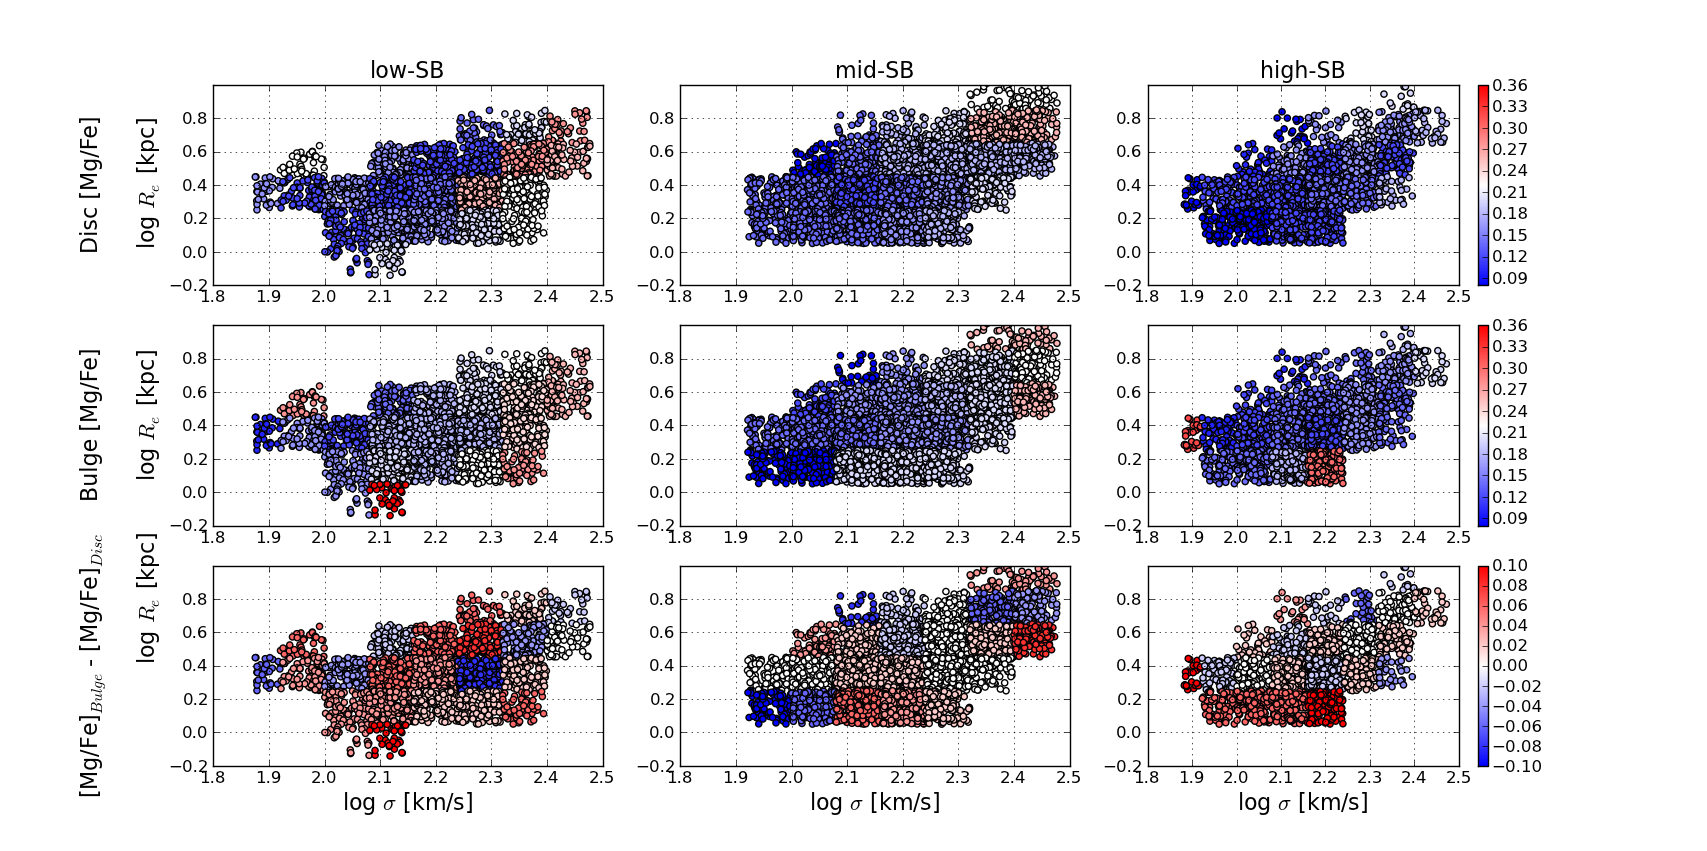
\includegraphics[scale=0.43]{MgFe_map_9panel.png}
\end{center}
\caption{The measurements of the [Mg/Fe] metallicities are represented by the colour of the data points. The redder a data point is, the higher value of [Mg/Fe]. This plot shows that [Mg/Fe] increases as $I_e$ decreases, as well as when $\sigma$ increases. Comparing the difference between the morphological types (row 3), it can be noted that there is typically no difference between the two. \label{fig:MgFe_maps}}
\end{figure}

\section{Discussion}

Bundy et al. (2010) claim that it is possible that disc morphological type galaxies on the red sequence are formed from disc type galaxies in the blue cloud where internal processes have quenched star formation. If this theory is correct, we would expect that the age in the stellar population of bulge type galaxies is older than the stellar population of the disc type galaxies. When measuring the ages of the different population types, we find that the ages of the two types of morphologies are about equal, suggesting that internal processes that quench star formation aren't necessarily a correct model for all galaxies evolving out of the blue cloud.

It is not only age that we find to be the same between the morphological types, but the metallicities also are the same. This suggests that, in the central bulges of quiescent galaxies, the stars have properties that are not affected by what is happening outside of the central bulge.  

\section{Conclusions}

We have used the stellar properties of nearby ($0.025 \leq z \leq 0.100$) quiescent galaxies to test the passive disc as a galactic evolutionary stage. Using galaxies that measured FP parameters to be nearly the same, we were able to conclude that there is no statistically difference between the stellar properties in the central bulge regions of red-sequence galaxies that show a prominent disc, and those that are dominated by their central bulge regions. More specifically:

\begin{enumerate}
\item The age difference between the bulge regions of the disc morphological type galaxies' stellar populations and the bulge dominated morphological types shows no statistical difference. The difference in ages, $\text{Age}_{Disc}-\text{Age}_{Bulge}$, came out to have a distribution characterized by a mean of $\mu=0.162\pm0.023\ \text{Gyr}$ with a standard deviation of $\sigma=1.655\ \text{Gyr}$. A graphical representation of the distribution of the difference between galaxies that occupied the same regions of FP space can be seen in the first panel of Figure~\ref{fig:Delta_hist}.
\item The iron abundances, [Fe/H], between the stellar populations in the bulge regions of the disc and bulge type morphological types also show no statistical difference. The difference, $\text{[Fe/H]}_{Disc}-\text{[Fe/H]}_{Bulge}$, between galaxies of the same FP parameters has a distribution described by a mean of $\mu=0.050\pm0.001$, a standard deviation of $\sigma=0.099$, and can be seen in a graphical representation by the histogram in the second panel of Figure~\ref{fig:Delta_hist}.
\item The magnesium to iron abundance ratios, [Mg/Fe], between the stellar population in the central bulge regions of the disc and bulge type morphological types, which occupy the same region of FP space, have a distribution with a mean of $\mu=-0.018\pm0.001$ with a standard deviation of $\sigma=0.064$, (see Figure~\ref{fig:Delta_hist}). This distribution also shows no statically significant difference between the stellar populations in the two morphological types.
\end{enumerate}

Also to note is that the previous trends in age, [Fe/H], and [Mg/Fe] are still shown to exist for both bulge and disc type galaxies. These trends are:

\begin{itemize}
\item Galaxies of higher surface brightness have younger stellar populations.
\item Galaxies occupying the same slices of surface brightness in the FP tend to have older stellar populations in higher regions of velocity dispersion.
\item Galaxies of similar surface brightness are shown to have the same stellar population age over a constant region of $R_e$.
\item Iron is more abundant in galaxies of higher surface brightness.
\item Galaxies occupying the same slices of surface brightness in the FP are more iron rich when the velocity dispersion is larger.
\item {[Mg/Fe] shows to have higher values for galaxies of lower surface brightness.}
\item Galaxies of the same surface brightness in FP space are shown to have larger values of [Mg/Fe] for higher values of $M_{dyn}$, which is mapped by $M_{dyn}\propto \sigma^2 \ R_e$.
\end{itemize}


\begin{figure}
\begin{center}
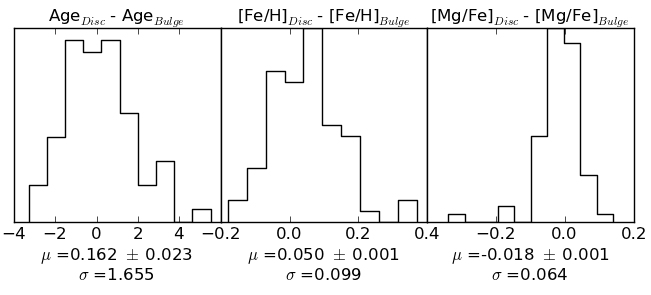
\includegraphics[scale=0.62]{3panel_Delta_hist.png}
\end{center}
\caption{The above histograms show the distribution of values for the difference in the stellar population properties explored in colour of the points in the third row of Figures~\ref{fig:age_maps}~,~\ref{fig:FeH_maps}~and~\ref{fig:MgFe_maps}. It can be noted that a value of zero for the mean, $\mu$, is within one standard deviation, $\sigma$, of the mean in all of the distributions. That is to say, that all the stellar population parameters explored in the central parts of different morphological types are the same when looking at quiescent galaxies that share the same FP parameters. The value for the uncertainty in the mean was calculated using Poisson statistics. That is to say, that it is equal to $\sigma/\sqrt{N}$, where $N$ is the number samples. \label{fig:Delta_hist}}
\end{figure}


\section{Acknowledgments}

I would first like to thank Genevieve Graves for all of her guidance during this entire research project. She has truly taught me how to approach scientific research in the field of astronomy. Secondly, I would like to acknowledge Patrick Fitzpatrick for his collaboration in classifying galaxies as red sequence, quiescent galaxies. Lastly, I would like to thank the astronomy department at the University of California, Berkeley for having great research opportunities for their undergraduate students.

\section{References}

Baldry, I. K., et al. 2004, ApJ, 600, 681

Bernardi, M. et al. 2006, AJ, 131, 2018

Bundy, K., et al. 2010, AJ, 719, 1969

Cheng, J. Y., et al. 2001, MNRAS, 412, 727

Djorgovski, S., \& Davis, M. 1987, ApJ, 313, 42

Faber, S. M. et al. 2007, ApJ, 665, 265

Gomez, P., et al. 2003, ApJ, 584, 210

Graves, G. J. \& Faber, S. M. 2010, ApJ, 717, 803

Graves, G. J., et al. 2010, ApJ, 721, 278

Graves, G. J. \$ Schiavon, R. P. 2008, ApjS, 177, 446

J\o gensen, I. et al. 1996 MNRAS, 280, 167

Schawinski, K. et al. 2009, MNRAS, 396, 818

Simard, L., et al. 2002, ApJs, 142, 1

Strateva, I., et al. 2001, AJ, 122, 1861

York, D. G., et al. 2000, AJ, 120, 1579



\end{document}
